\documentclass[11pt]{exam}
\usepackage[spanish]{babel}
\usepackage[utf8]{inputenx}
\usepackage{fontenc}
\usepackage{textcomp}
\usepackage{lmodern,pifont}
\usepackage{graphicx}
\graphicspath{ {./img_1479/} }
\usepackage{setspace}
\usepackage[dvipsnames]{color}
\usepackage{colortbl}
\usepackage{caption}
\usepackage{amsmath}

\newcommand\titexam[1]{\centering%
\fbox{\parbox{\textwidth}{\huge \sffamily \textbf{#1}}}\normalsize \vspace{1em}}

\renewcommand{\solutiontitle}{\noindent\textbf{Solución:}\par\noindent}

\pagestyle{empty}
\begin{document}
{\fontfamily{lmss}\selectfont
\textbf{INSTRUCCIONES:}
\begin{itemize}
    \item Se dispone de dos horas para responder las 20 preguntas.
    \item Cada pregunta tiene un valor de 0.5 punto.
    \item Para considerar la respuesta como correcta, la opción escogida ha de
      estar correctamente señalada. Las preguntas erróneamente marcadas se
      considerarán como incorrectas. 
    \item Cada respuesta incorrecta resta 0.17 puntos. Las respuestas en blanco no restan. 
\end{itemize}
\vspace{1cm}

\titexam{MF1479\_2 Propagación de plantas en vivero}

\begin{questions}
  % 1
\question Señala cuál de las siguientes especies son coníferas
\begin{checkboxes}
  \choice A. Plataneros, encinas y robles
  \choice B. Pinos, cedros y abetos
  \choice C. Enebros, sabinas y cipreses
  \CorrectChoice D. Las respuestas B y C son correctas
\end{checkboxes}
% 2
\question ¿Qué ecosistemas son extremadamente sensibles a la contaminación por
  plantas invasoras y con las que hay que hay que extremar precauciones?
  \begin{checkboxes}
    \choice A. Ecosistemas de montaña
    \CorrectChoice B. Ecosistemas de agua dulce (ríos y sus
    riveras, lagos, humedales, etc)
    \choice C. Ecosistemas dunares
    \choice D. Ecosistema forestal
  \end{checkboxes}
% 3
% \question ¿Como se llama la parte de la flor donde se forma y almacena el polen?
%   \begin{checkboxes}
%     \choice A. Cáliz
%     \CorrectChoice B. Estambre
%     \choice C. Tubo polínico
%     \choice D. Gineceo
%   \end{checkboxes}
\question ¿La vermiculita es un tipo de sustrato?
  \begin{checkboxes}
    \choice A. Un sustrato orgánico
    \CorrectChoice B. Un sustrato inorgánico transformado
    \choice C. Un sustrato de origen natural de origen inorgánico
    \choice D. Ninguna respuesta es correcta 
  \end{checkboxes}
%  4
\question Los nutrientes de un suelo se clasifican en macroelementos y microelementos. ¿A
  qué se debe el nombre de estos últimos?
  \begin{checkboxes}
    \choice A. A qué la mayoría de elementos son de pequeño tamaño
    \choice B. A qué tienen poca importancia para las plantas
    \choice C. A qué se encuentran en el suelo en poca proporción
    \CorrectChoice D. A qué se encuentran en las plantas en menor proporción 
  \end{checkboxes}
  \newpage
% 5
\question Las fertilizaciones en un suelo pueden ser minerales u orgánicas. ¿Qué tipo
  de fertilizantes se emplean en la fertilización orgánica?
  \begin{checkboxes}
    \choice A. Estiércol, humus de lombriz o NPK inorgánico
    \choice B. Abono verde  o enmiendas calizas
    \CorrectChoice C. Estiércol, humus, compost, guano, gallinaza, abono verde
    \choice D. Las respuestas A y B son correctas
  \end{checkboxes}
% 6
\question El objetivo principal de la preparación de suelos es provocar transformaciones
  que mejoren la germinación y el desarrollo de las plantas. ¿Las preparaciones que se
  realizan pueden conseguir fines como?
  \begin{checkboxes}
    \choice A. Aireación del suelo y/o destrucción de hierbas no deseadas
    \choice B. Aportaciones de nutrientes o enmiendas para mejorar la calidad del suelo
    \choice C. Eliminación de actividad microbiana
    \CorrectChoice D. Las respuestas A y B son correctas
  \end{checkboxes}
% 7
\question ¿Qué propiedad física del suelo depende del tamaño de las partículas que la
  componen?
  \begin{checkboxes}
    \CorrectChoice A. Textura
    \choice B. Porosidad
    \choice C. Estructura
    \choice D. Ninguna respuesta es correcta
  \end{checkboxes}
% 8
\question Como afecta el pH del suelo a los elementos químicos presentes en el suelo?
  \begin{checkboxes}
    \choice A. Con pH más ácidos la mayoría de los nutrientes serán absorbidos más
    fácilmente
    \choice B. Afecta a la disponibilidad de nutrientes para las plantas.
    \choice C. Dependiendo del pH del suelo algunos nutrientes serán más fácilmente
    absorbidos por las plantas que otros
    \CorrectChoice D. Las respuestas B y C son correctas
  \end{checkboxes}
% 9
\question ¿Qué tipo de raíz aparece en la imagen?
  \begin{figure}[h!]
    \centering
    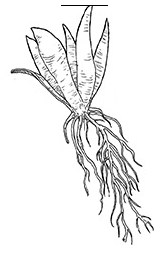
\includegraphics[width=0.2\textwidth]{fasciculada.PNG}
  \end{figure}
  \begin{checkboxes}
    \choice A. Napiforme
    \choice B. Pivotante
    \choice C. Ramificada
    \CorrectChoice D. Fasciculada
  \end{checkboxes}
% 10
\question La frase: \emph{``La ropa de trabajo corriente es un EPI fundamental''}, ¿es?
  \begin{checkboxes}
    \CorrectChoice A. Falsa
    \choice B. Falsa. Solo es un EPI fundamental si los pantalones son largos
    \choice C. Verdadera
    \choice D. Verdadera solo si el operario la utiliza correctamente
  \end{checkboxes}
 
  % 11
  \question ¿Qué consecuencias podría tener un suelo en el que hubiera un exceso
  de poros de gran tamaño?
  \begin{checkboxes}
    \choice A. Que fuese un suelo pesado en el que las raíces se desarrollaran
    con dificultad
    \CorrectChoice B. Un suelo muy suelto que se secase rápidamente
    \choice C. Una labranza dificultosa
    \choice D. Un suelo con una óptima capacidad de retención de agua
  \end{checkboxes}
% \question ¿Los tipos de riesgos que un operario corre por  realizar tareas de abonado del
%   terreno pueden ser?
%   \begin{checkboxes}
%     \choice A. Sobreesfuerzos por manipular cargas o posturas inadecuadas
%     \choice B. Contacto con agentes químicos o ingestión accidental de tóxicos
%     \choice C. Lesiones en la piel por salpicaduras de residuos o agentes químicos
%     \CorrectChoice D. Todas las respuestas son correctas
%   \end{checkboxes}
  % 12
\question ¿Qué es un tratamiento pregerminativo de semillas?
  \begin{checkboxes}
    \choice A. Una técnica que mejora la calidad de las semillas
    \CorrectChoice B. Un conjunto de técnicas que han de facilitar el germinado de las
    semillas
    \choice C. Un conjunto de técnicas que aumentan el vigor de las semillas
    \choice D. Todas las respuestas son correctas
  \end{checkboxes}
  % 13
\question Además de poder controlar la presencia de hierbas no deseadas de forma manual o
  mecánica, ¿de qué otra manera podemos evitar la presencia de hierbas no deseadas sin
  emplear herbicidas?
  \begin{checkboxes}
    \choice A. Arranque
    \choice B. Siega
    \CorrectChoice C. Mulching o acolchados
    \choice D. Fumigando
  \end{checkboxes}
  % 14
\question ¿El tegumento o epispermo es una parte de?
  \begin{checkboxes}
    \choice A. De un fruto
    \CorrectChoice B. De una semilla
    \choice C. Es un tipo de polinización
    \choice D. Es la reserva de alimento de una semilla
  \end{checkboxes}
  % 15
\question ¿La estratificación consiste en?
  \begin{checkboxes}
    \choice A. Un tratamiento pregerminativo
    \choice B. Colocar las semillas embebidas en agua o en estratos húmedos
    \choice C. Alterar el tegumento de las semillas
    \CorrectChoice D. Las respuestas A y B son correctas
  \end{checkboxes}
  % 16
\question Las plantas tienen capacidad de reproducirse de manera asexual mediante
  ciertas estructuras tales como?
  \begin{checkboxes}
    \CorrectChoice A. Bulbos y tubérculos
    \choice B. Estacas y esquejes
    \choice C. Acodo y rizoma
    \choice D. Todas las respuestas son correctas 
  \end{checkboxes}
  % 17
% \question ¿Cuantas yemas debe contener como mínimo un esqueje o estaquilla para un correcto
%   desarrollo y enraizado?
%   \begin{checkboxes}
%     \choice A. No importa el número de yemas, solo la calidad de la planta madre
%     \choice B. Una
%     \CorrectChoice C. Dos
%     \choice D. Con una yema será suficiente siempre y cuando dejemos las hojas completas
%   \end{checkboxes}
\question ¿Como se llama el órgano de reproducción subterráneo que está formado
  por un engrosamiento de las raíces?
  \begin{checkboxes}
    \CorrectChoice A. Tubérculo
    \choice B. Rizoma
    \choice C. Estolones
    \choice D. Bulbo    
  \end{checkboxes}
  % 18
\question ¿Como se llama la técnica de reproducción vegetativa en la que se
  fuerza a un tallo a emitir raíces adventicias cubriéndolo con tierra?
  \begin{checkboxes}
    \choice A. Injerto
    \CorrectChoice B. Acodo
    \choice C. Estaquillado
    \choice D. Estolonado
  \end{checkboxes}
  % 19
\question Al reproducir plantas mediante estaquillas hay que tomar medidas que prevean el
  desecamiento de las estaquillas. ¿Qué medidas son adecuadas?
  \begin{checkboxes}
    \choice A. Aumentar la iluminación
    \CorrectChoice B. Emplear sistemas de nebulización y/o cultivar debajo de túneles de
    plástico
    \choice C. Ventilar por las noches
    \choice D. Aumentar la  temperatura de la parte aérea
  \end{checkboxes}
  % 20
\question ¿Qué es un patrón?
  \begin{checkboxes}
  \choice A. Persona encargada de los trabajos en el campo
  \CorrectChoice  B. Planta que recibe un injerto y aporta el sistema radicular
  \choice C. Trozo de rama que se introduce en un pie o planta para reproducirla
  \choice D. Parte de una rama en la que hacemos una incisión para quitar un
  anillo y que cubrimos con sustrato ayudándonos de una bolsa.
  \end{checkboxes}
\end{questions}}

\end{document}
%%% Local Variables:
%%% mode: latex
%%% TeX-master: t
%%% End:
